% Opcje klasy 'iithesis' opisane sa w komentarzach w pliku klasy. Za ich pomoca
% ustawia sie przede wszystkim jezyk i rodzaj (lic/inz/mgr) pracy, oraz czy na
% drugiej stronie pracy ma byc skladany wzor oswiadczenia o autorskim wykonaniu.
\documentclass[polish,inz,shortabstract,declaration]{iithesis}

\usepackage[utf8]{inputenc}
\usepackage{graphicx,listings,amsmath,amsthm,amsfonts}
\usepackage{subcaption}
\usepackage{lipsum}
\usepackage{xargs}
\usepackage[usenames,dvipsnames]{xcolor}
\usepackage[colorinlistoftodos,prependcaption,textsize=tiny,shadow]{todonotes}
\usepackage{booktabs}

\newcommandx{\unsure}[2][1=]{\todo[linecolor=red,backgroundcolor=red!25,bordercolor=red,#1]{#2}}
\newcommandx{\change}[2][1=]{\todo[linecolor=blue,backgroundcolor=blue!25,bordercolor=blue,#1]{#2}}
\newcommandx{\info}[2][1=]{\todo[linecolor=OliveGreen,backgroundcolor=OliveGreen!25,bordercolor=OliveGreen,#1]{#2}}
\newcommandx{\improvement}[2][1=]{\todo[linecolor=purple,backgroundcolor=purple!25,bordercolor=purple,#1]{#2}}
\newcommandx{\add}[2][1=]{\todo[linecolor=Goldenrod,backgroundcolor=Goldenrod!25,bordercolor=Goldenrod,#1]{#2}}
\newcommandx{\thiswillnotshow}[2][1=]{\todo[disable,#1]{#2}} 

\polishtitle    {Zastosowanie auto-enkoderów wariacyjnych do rozpoznawania zmian na obrazach medycznych}
% \englishtitle   {English title}

\author         {Tomasz Nanowski}
\advisor        {dr Jan Chorowski}
%\date           {}
\transcriptnum  {279076}                     
\advisorgen     {dr. Jana Chorowskiego}

 \polishabstract {Problemem, który zainspirował mnie do napisania tej pracy było lokalizowanie zmian nowotworowych w zdjęciach wykonanych metodą rezonansu magnetycznego. O ile można podejść do tego zadania od strony nadzorowanej, czyli bazowania na danych przeanalizowanych wcześniej przez specjalistów, gdzie każdy przypadek musiał zostać ręcznie obejrzany i oznaczony, to mimo wielu jego zalet jak chociażby korzystanie z rzeczywistej wiedzy eksperckiej, zbiór taki jest bardzo kosztowny w przygotowaniu i dalszym rozwoju, a dodatkowo jest on ograniczony do przykładowo pojedynczej partii ciała. Zauważając te wady oraz łącząc je z obserwacją, że zmiany patologiczne tak na prawdę są rzadkie i są pewnym odstępstwem od normy, chciałem spróbować skorzystać z metody nienadzorowanej, w której to model nauczyłby się oszacowywać prawdopodobieństwo występowania pojedynczej próbki w pewnym kontekście. Przy takim podejściu mógłbym oznaczać obserwacje mało prawdopodobne jako właśnie te nowotworowe. Model, który zdecydowałem się wykorzystać do tego zadania to autoenkoder wariacyjny (ang. Variational Autoencoder), łączący sztuczne sieci neuronowe z modelowaniem probabilistycznym. Pomysł przetestowałem początkowo na danych syntetycznych, wykorzystując do tego zbiór MNIST. Otrzymane wyniki okazały się być zadowalające i zachęcały do przeprowadzenia dalszych eksperymentów już na danych medycznych. Niestety w tym przypadku nie można było uznać tego za sukces, a według mojej analizy model nauczył się jedynie zwracać uwagę na prostą własność, jaką jest jasność próbki. Na tym zakończyłem moją pracę i przygotowałem propozycje rozwiązań, które mogłyby według mnie pozytywnie wpłynąć na poprawę rezultatów.}


\begin{document}

\listoftodos[Notes]

\chapter{Introduction}

 Czy wykorzystanie sztucznych sieci neuronowych może pomóc w diagnozowaniu nowotworów? W tej pracy będę chciał przedstawić podejście do tego problemu z wykorzystaniem wariacyjnego auto-enkodera. Dane na których będę bazował pochodzą z uniwersytetu Duke i przedstawiają zdjęcia rezonansowe głowy pacjentów z wykrytym nowotworem. I tu pojawia się jeden z pierwszych problemów, jakim jest niezbalansowanie danych. W ogólności liczba osób chorych jest zdecydowanie mniejsza od tych zdrowych, a dodatkowo samych komórek nowotworowych też jest mniej w porównaniu do pozostałych. W tym ma właśnie pomóc VAE, który stara się oszacować prawdopodobieństwo wystąpienia danej próbki, a skoro danych zmutowanych jest mniej, to ich prawdopodobieństwo również powinno być niższe. Będzie to jedna z podstaw użyta do klasyfikowania występowania raka.

%Can the use of artificial neural networks help diagnose cancer? In this work, I am going to present an approach to this problem using a Variational Autoencoder. The data on which I will be based come from the University of Duke and present resonant images of the head of patients with detected cancer. And here comes one of the first problems, which is the unbalancing of data. In general, the number of patients is much smaller than the healthy ones, and in addition, the cancer cells themselves are also less compared to the others. This is to be helped by VAE, which tries to estimate the probability of a given sample, and since the mutant data is less, their likelihood should also be lower.
\chapter{Experiments on MNIST}

Na początek chciałbym zacząć od odtworzenia docelowego problemu na prostszych danych jakim jest zbiór MNIST. Pozwoli to w ogólności stwierdzić sensowność skorzystania z wybranego modelu. Zakładam, że jeśli eksperyment nie powiódłby się na łatwiejszych danych, to raczej nie powiedzie się również na tych bardziej skomplikowanych. To miejsce traktuje jako poligon testowy. Pozwoli mi to też nabrać pewnego rodzaju doświadczenia z wybranym modelem.

Sytuację, którą będę chciał poddać testowi jest całkowite niezbalansowanie danych, a wręcz brak danych drugiej kategorii i obserwacja jak zachowuje sie w takim przypadku model. Będę chciał to osiągnąć poprzez uczenie modelu jedynie na danych pochodzących z dwóch klas [4, 7], a następnie obserwacja tego co się stanie z modelem przy zaaplikowania danych z klasy [5]. Ma to odtworzyć sytuację gdzie danych opisujących zmiany nowotworowe jest przytłaczająco mniej od tych zdrowych.

\section{MNIST}

Jest to zbiór po kategoryzowanych odręcznie napisanych cyfr. Wszystkie obrazki są czarno-białe, rozmiaru 28x28 i wycentrowane. Każdy piksel ma wartość dualną: 0 albo 1. Zbiór składa się z 60000 danych treningowych i 10000 testowych. Przykładowe obrazki \ref{fig:mnist}.

\begin{figure}[h!]
    \centering
    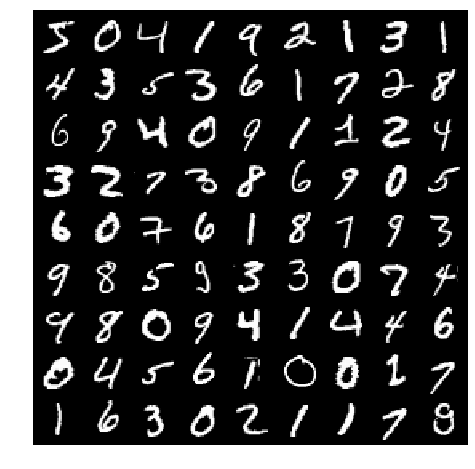
\includegraphics[width=0.4\textwidth]{images/mnist}
    \caption{Samples from MNIST dataset}
    \label{fig:mnist}
\end{figure}

\section{VAE}

Na rysunku \ref{fig:vae} znajduje się efekt wyuczenia modelu VAE z warstwą ukrytą rozmiaru 20. Po lewej widać rekonstrukcje, a po prawej efekty zdekodowania wektora wygenerowanego ze standardowego rozkładu normalnego.

\begin{figure}[h!]
  \centering
  \begin{subfigure}[b]{0.57\linewidth}
    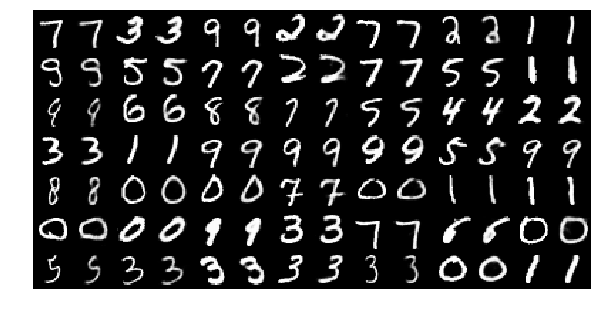
\includegraphics[width=\linewidth]{images/mnist_recon}
    \caption{W nieparzystych kolumnach znajdują się oryginalne obrazki, natomiast po prawej ich rekonstrukcje}
  \end{subfigure}
  \begin{subfigure}[b]{0.30\linewidth}
    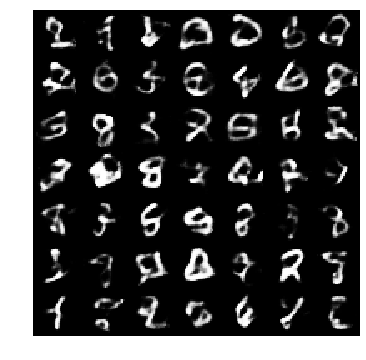
\includegraphics[width=\linewidth]{images/mnist_gen}
    \caption{Przykłady wygenerowanych obrazków}
  \end{subfigure}
  \caption{Przedstawienie efektów modelu VAE}
  \label{fig:vae}
\end{figure}

Dodatkowo warto byłoby zobaczyć jak konkretne cyfry rozrzucane są w przestrzeni. 20 wymiarów jest dosyć trudne do zwizualizowania, więc wyuczyłem model dla reprezentacji ukrytej rozmiaru 2. Na rysunku \ref{fig:mnist_2d} znajdują sie wyniki. Wartym odnotowania jest fakt, że niektóre klasy są bardzo dobrze separowalne. Widać tu właśnie opisane wcześniej zalety modelu VAE. Te ciekawą własność wyniku reprezentacji będę chciał wykorzystać w późniejszej analizie.

\begin{figure}[h!]
    \centering
    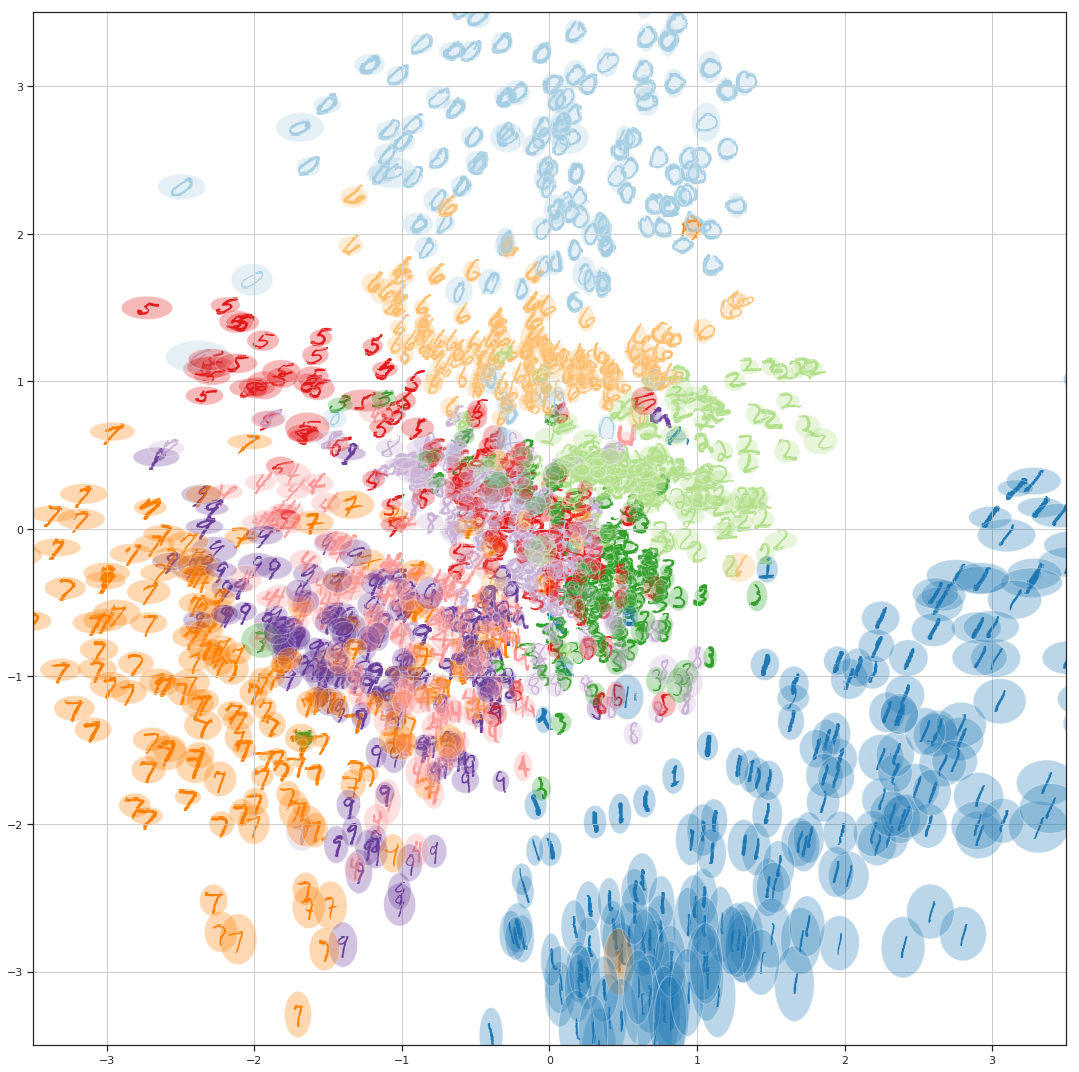
\includegraphics[width=1.\textwidth]{images/mnist_2d}
    \caption{}
    \label{fig:mnist_2d}
\end{figure}

W oryginalnym problemie mamy bardzo duży dysonans pomiędzy ilością przykładów dla każdej z klas. Według statystyk dane z komórkami rakowymi stanowią ~1\% wszystkich. Ciężko jest wiec nawet mówić o jakimś sensownym podejściu supervised. Do zasymulowania tego problemu dla MNIST będę uczył model jedynie na dwóch klasach [4, 7], a następnie testował zachowanie reprezentacji ukrytej dla przekładów z klasy 5.

Rozmiar reprezentacji ukrytej wynosi 10. Analizować natomiast będziemy 2 składowe kosztu dla modelu VAE: KLD oraz błąd rekonsrukcji MSE. Na rysunku \ref{fig:mnist_compare} znajduje się przedstawienie ich wraz z histogramami. Można zauważyć, że wyłącznie na podstawie samego błędu rekonstrukcji można z bardzo dużą dokładnością określić dane pochodzące z klasy 5, mimo iż model nie widział żadnych ich przykładów podczas uczenia.

\begin{figure}[h!]
    \centering
    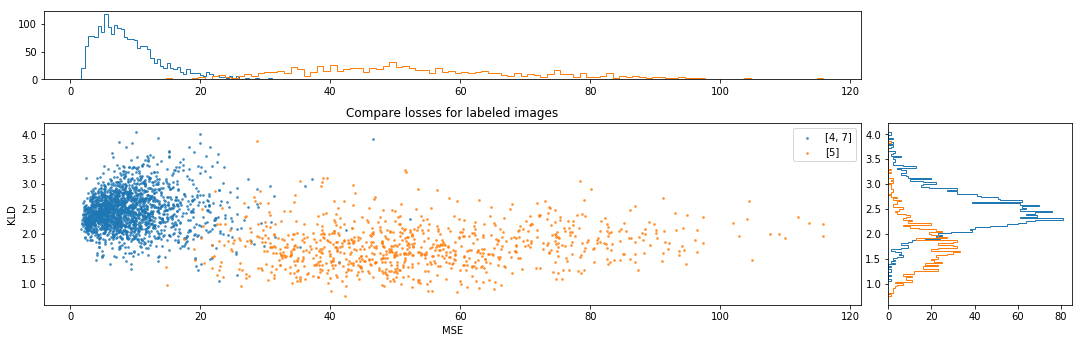
\includegraphics[width=1.0\textwidth]{images/mnist_compare}
    \caption{}
    \label{fig:mnist_compare}
\end{figure}

Do określenia jak rzeczywiście dobra jest ta separacja można wykorzystać krzywą ROC. Traktujemy to jako problem binarnej klasyfikacji, gdzie dane z klasy 5 będą oznaczone jako 1, a z [4, 7] jako 0. Wartość confidence to suma kosztów KLD i MSE. Jak widać na rysunku \ref{fig:mnist_roc} takie podejście osiąga prawie 100\% skuteczność. Podobne podejście będę chciał zastosować do danych medycznych.

\begin{figure}[h!]
    \centering
    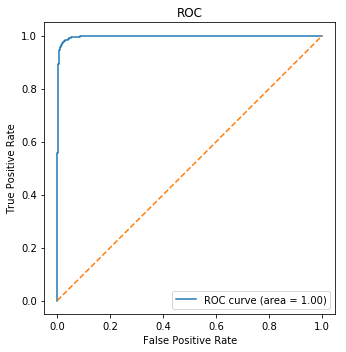
\includegraphics[width=0.5\textwidth]{images/mnist_roc}
    \caption{}
    \label{fig:mnist_roc}
\end{figure}

\subsection{Krzywa ROC i AUC}

Krzywa ROC (Receiver Operating Characteristic) jest narzędziem do oceny poprawności klasyfikatora binarnego. Bazuje ona na wyliczaniu charakterystyki jakościowej modelu predykcji w wielu różnych punktach odcięcia. Z praktycznego punktu widzenia działa to na takiej zasadzie, że mamy dane pochodzące z dwóch klas. Model odpowiada z jaką pewnością dane należą do klasy 1. Następnie badamy różne progi i klasyfikujemy obiekty (jeśli przewidziana wartość jest powyżej progu to 1 wpp 0). Dla uzyskanych klasyfikacji liczymy TPR oraz FPR i nanosimy te wartości na wykres. Warto zauważyć, że dla losowego modelu jego wykres to prosta przechodząca przez (0, 0) i (1, 1). Dzieje się tak, ponieważ w przy każdym progu połowa danych będzie nad i połowa pod. Idealny model znajduje się w punkcie (0, 1).

Przydatne jest również obliczenie pola powierzchni pod krzywą AUC (Area Under Curve). Interpretuje się ją jako prawdopodobieństwo, że badany model predykcyjny oceni wyżej losowy element klasy pozytywnej od losowego elementu klasy negatywnej.

\section{Deep feature consistent variational auto-encoder}

Podobny eksperyment jw. przeprowadziłem również dla modelu DFC. Na początku jednak warto zobaczyć co zyskujemy na zmianie podejścia do kosztu rekonstrukcji. Różnice prezentują się na rysunku \ref{fig:vae_dfc_recon}. Widać, że rekonstrukcje są mniej rozmazane niż przy standardowym VAE. Dodatkowo lepiej rekonstruuje takie elementy jak np. pozioma kreska w cyfrze 7. 

\begin{figure}[h!]
    \centering
    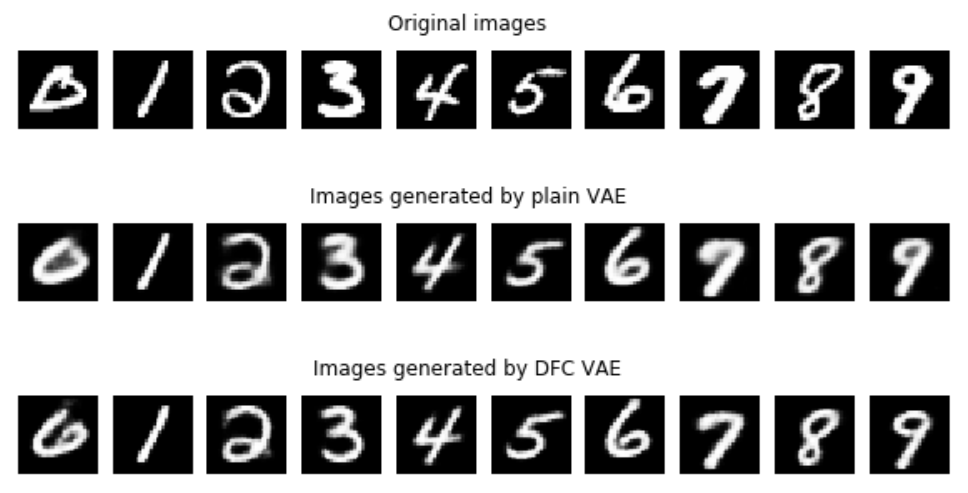
\includegraphics[width=0.8\textwidth]{images/vae_dfc_gen}
    \caption{}
    \label{fig:vae_dfc_recon}
\end{figure}

Na rysunku \ref{fig:dfc_mnist_compare} przedstawiony jest efekt przeprowadzenia analogicznego eksperymentu z nauką na jedynie przykładach z klas [4, 7] i sprawdzeniu zachowania dla danych z klasy 5. Zamiast kosztu rekonstrukcji MSE używamy błędu perceptualnego. Dodatkowy model splotowy również nie widział danych pochodzących z 5 klasy. Jak widać separacja jest co najmniej tak dobra jak w przypadku zwykłego VAE.

\begin{figure}[h!]
    \centering
    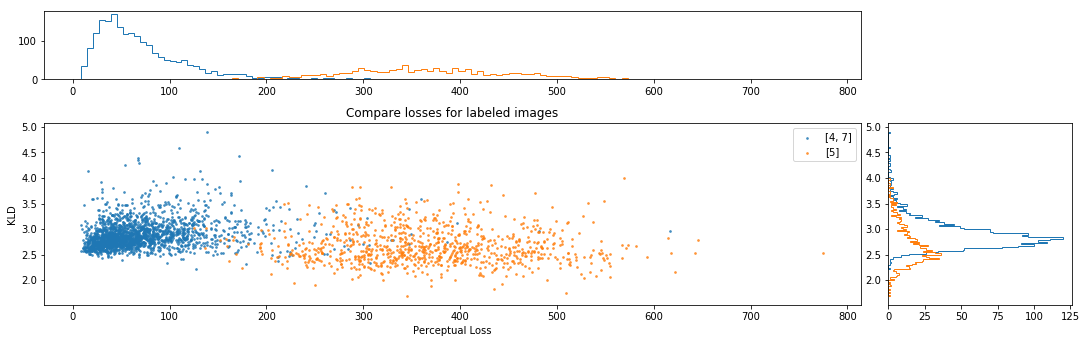
\includegraphics[width=1.0\textwidth]{images/dfc_mnist_compare}
    \caption{}
    \label{fig:dfc_mnist_compare}
\end{figure}

\chapter{Eksperyment na danych właściwych (MRI FLAIR)}

\section{Opis danych}

Dane pochodzą z Uniwersytetu Duke'a (ang. Duke University). Są to zdjęcia głowy wykonane metodą obrazowania rezonansu magnetycznego w technice FLAIR (ang. fluid-attenuated inversion recovery) wraz z zaznaczonymi obszarami zmian nowotworowych. Obrazy mają rozmiar 256x256x3 pikseli, gdzie pierwszy kanał odpowiada momentowi przed wprowadzeniem kontrastu, trzeci po, a drugi jest właściwym zdjęciem. Maski mają rozmiar 256x256 pikseli o wartościach odpowiednio 255 dla komórek nowotworowych i 0 w przeciwnym wypadku. Na rysunku \ref{fig:medical_description} pokazane są zdjęcia z podziałem na kanały i odpowiadające im maski.

\begin{figure}[h!]
    \centering
    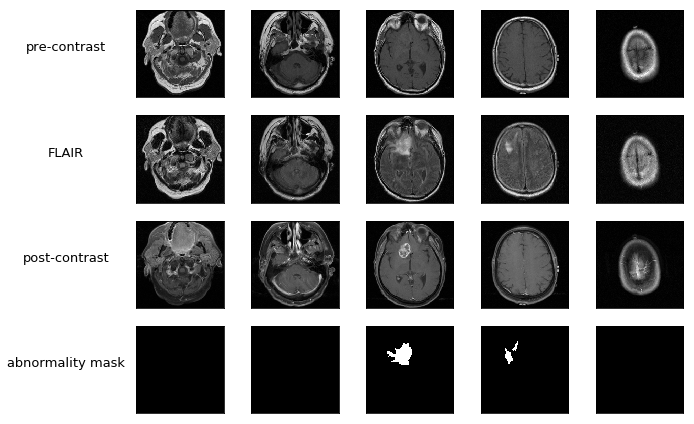
\includegraphics[width=0.8\textwidth]{images/medical_description}
    \caption{Przedstawienie konkretnych kanałów w próbce wraz z jego maską zmian}
    \label{fig:medical_description}
\end{figure}

Dane pogrupowane są dla 110 pacjentów ze zdiagnozowanym nowotworem. Na rysunku \ref{fig:medical_sample} zaprezentowałem zdjęcia pojedynczej osoby w trzech kanałach. Łącznie w zbiorze danych znajduje się 3929 par obrazów, przy czym jedynie $\sim1.02988\%$ pikseli zostało zidentyfikowanych jako komórki nowotworowe, co potwierdza obserwację odnośnie ich rzadkości.

\begin{figure}[h!]
    \centering
    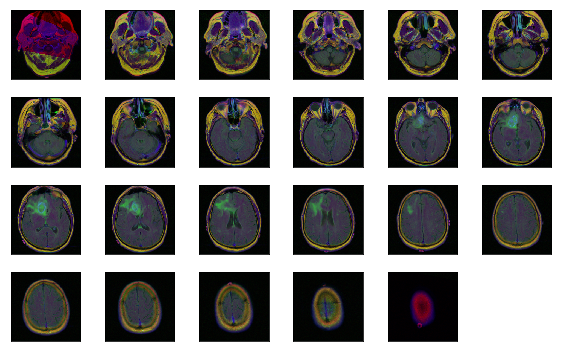
\includegraphics[width=0.8\textwidth]{images/medical_sample}
    \caption{Przykładowy zestaw obrazków dla pojedynczego pacjenta}
    \label{fig:medical_sample}
\end{figure}

\section{Wstępna obróbka}

Dane podzieliłem na 2 rozłączne zbiory ze względu na pacjentów w stosunku 70\% dla zestawu treningowego i 30\% dla testowego.

\subsection{Podział na mniejsze kawałki}

Danymi, które rzeczywiście mnie interesują są poszczególne komórki w mózgu. To co chciałbym umieć oceniać to ich patologiczność. Mam zamiar to robić na podstawie kontekstu w jakim się znajdują, czyli lokalnego sąsiedztwa na zdjęciu. W praktyce sprowadzi się to do utożsamiania wycinka obrazu rozmiaru $n$ x $n$ z wartością komórki leżącą w jego środku. W takim sensie chce podzielić zbiór danych na mniejsze kawałki, żeby każdej komórce odpowiadał jej kontekst. Jednak parametrem wymagającym ustalenia jest rozmiar takiego sąsiedztwa. Musze wiedzieć czy kawałek o danych wymiarach będzie zawierał wystarczającą ilość informacji potrzebnych do poprawnej klasyfikacji. Teoretycznie za kontekst mógłbym uznać cały obrazek, ale zależy mi też na ograniczeniu rozmiaru modelu i potrzebnej w związku z tym mocy obliczeniowej. Do wyznaczenia tej wartości skorzystam z podejścia nauki nadzorowanej, co może wydawać się sprzeczne z moją początkową deklaracją, ale ten krok służy jedynie we wsparciu wyboru optymalnego rozmiaru i nie jest wymagany.

Decyzję podejmę na podstawie rezultatów osiąganych przez modele takie jak regresja liniowa oraz splotowa sieć neuronowa dla następujących rozmiarów: 16, 22, 28, 32, 48, 64. Zakładam, że jeśli w jakimś przypadku dokładność będzie zadowalająca, to ilość obecnych informacji wystarczy do rekonstrukcji. Warto w tym miejscu wspomnieć, że przy takim podejściu muszę zrównoważyć dane w zbiorze treningowym, ponieważ aktualnie jednych jest około 100 razy mniej niż drugich. Rozwiążę to na takiej zasadzie, że w trakcie uczenia porcję danych wejściowych będę komponował losując połowę próbek z jednej klasy i połowę z drugiej. Może to wpłynąć negatywnie na obciążenie modelu, ale i tak ostateczna klasyfikacja będzie odbywać się z wykorzystaniem progu, co powinno zredukować ten błąd. Wyniki zaprezentowałem przy pomocy krzywych ROC na wykresie \ref{fig:supervised_patches}. Jak można zauważyć wszystkie rozważane rozmiary prezentują się równie dobrze, w związku z czym zdecydowałem się wybrać jako parametr liczbę 22.

\begin{figure}[h!]
  \centering
  \begin{subfigure}[b]{0.45\linewidth}
    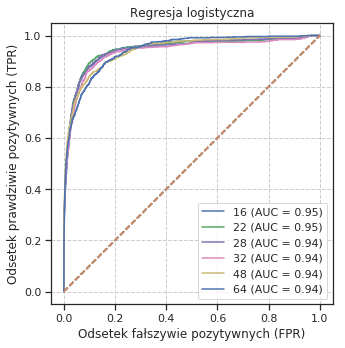
\includegraphics[width=\linewidth]{images/logreg_patch_roc_v2}
    %\caption{}
  \end{subfigure}
  \begin{subfigure}[b]{0.45\linewidth}
    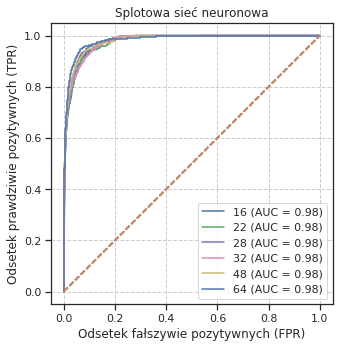
\includegraphics[width=\linewidth]{images/cnn_patch_roc_v2}
    %\caption{}
  \end{subfigure}
  \caption{Porównanie dokładności ze względu na różne rozmiary wycinków dla modeli uczonych metodą nadzorowaną}
  \label{fig:supervised_patches}
\end{figure}

Nie jest to oczywiście najlepsza metoda dla podejścia nadzorowanego, czym mogłoby być wykorzystanie architektury U-Net, ale powinno wystarczyć jako punkt odniesienia dla wymaganej ilości informacji w wycinku.

Dodatkowo w tym miejscu chciałbym wprowadzić słownictwo jakie będę używał do określania konkretnych próbek. Te odnoszące się da zmian nowotworowych będę nazywał pozytywnymi, a pozostałe negatywnymi.

\subsection{Dodatkowe analiza zbioru}

Po zdecydowaniu się na łatki rozmiaru 22 i przygotowaniu takiego zbioru postanowiłem dodatkowo przeanalizować jego zawartość w celu znalezienia trywialnych przypadków. Jednym z nich były kawałki znajdujące się poza czaszkę, które nigdy nie są nowotworowe. Będą to obrazki o niskiej łącznej sumie pikseli, co zaprezentowane jest na histogramie \ref{fig:pixel_sums}. Na początku można zauważyć sporą grupę przypadków niepatologicznych. Sprawdziłem, że minimalna wartość sumy dla klasy odpowiadającej nowotworom wynosi $56.5$. Przy tym założeniu usunąłem wszystkie obrazki u sumie mniejszej, niż $42.0$ co zmniejszyło ilość danych o $45.5\%$, pozbywając się trywialnych próbek. Dany próg będę oczywiście uwzględniał w późniejszej klasyfikacji.

\begin{figure}[h!]
    \centering
    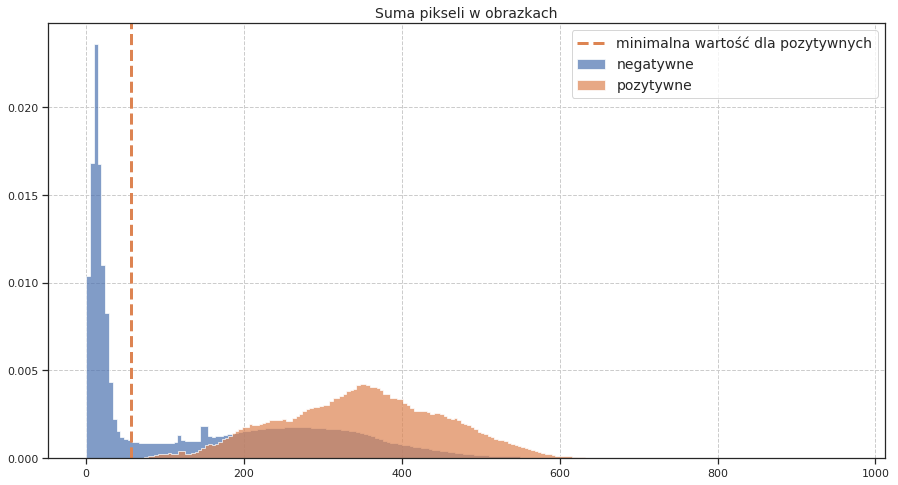
\includegraphics[width=1.0\textwidth]{images/pixel_sums_v3}
    \caption{Znormalizowany rozkład sum pikseli dla poszczególnych rodzajów próbek}
    \label{fig:pixel_sums}
\end{figure}

\section{Wyniki}

Przetestuje 4 kombinacje modeli, ze zmienioną funckją kosztu

W tabeli \ref{table:results} zostały przedstawione wyniki dla czterech kombinacji modeli oraz parametrów. Wartości liczbowe opisują najlepsze AUC ROC podczas uczenia wraz z odpowiadającą epoką. Jak widać w tym zestawieniu najlepiej wypadły podstawowe modele VAE.

\begin{table}[h!]
	\centering
    \begin{tabular}{ l | c c c c c c }
 
    \multicolumn{1}{c}{Model} & \multicolumn{6}{c}{Epoka} \\
    \cmidrule(r){1-1} \cmidrule(r){2-7}
    %\toprule
     		& 1 & 2 & 3 & 20 & 60 & 80 \\ \cmidrule(r){2-7}
    VAE 20-d 	& 0.494 & 0.693 & 0.655 & 0.612 & 0.597 & 0.590 \\ \hline
    VAE 50-d 	& 0.552 & 0.686 & \textbf{0.711} & 0.616 & 0.606 & 0.592 \\ \hline
    VAE 100-d 	& 0.580 & 0.685 & 0.650 & 0.614 & 0.595 & 0.594 \\ \hline
    VAE 200-d   & 0.661 & 0.675 & 0.668 & 0.620 & 0.608 & 0.597 \\ \hline
    VAE 300-d   & 0.704 & 0.671 & 0.657 & 0.620 & 0.600 & 0.593 \\
    \toprule
    \end{tabular}
    \caption{AUC przy danym modelu w danej epoce}
	\label{table:results}
\end{table}
\improvement{Dodać z-dim}

\section{Analiza}

Zajmę się analizą modelu w wersji VAE + Softmax. Na wykresie \ref{fig:soft_vae} przedstawione są koszty, ich rozkłady, przykłady rekonstrukcji oraz krzywa ROC. Ciekawie wyglądają te dwa zauważalne ogony na wykresie. Postaram sie lepiej przyjrzeć ich specyfice. 

Pierwszym pomysłem jest, żeby sprawdzić rozkład obrazków w zależności od ich jasności, czyli łącznej sumy pikseli. Ciemne obrazki defiuniuje jako te o niskiej sumie, a jasne o wysokiej. Na rysunku \ref{fig:soft_vae_th} zaznaczyłem negatywne obrazki, dla których suma <= 50 oraz pozytywne obrazki z sumą co najmniej 150. Zaznaczone śa one odpowiednio zielonym i czerwonym kolorem na wykresie. Jak widać po rozkładach składają się one na dokładnie te 2 separowalne ogony. Wniosek z tego jest następujący. Na podstawie tego modelu możemy odesparować jedynie najciemniejsze i najjaśniejsze obrazki z obydwu klas. W takim razie model nie robi nic nadzwyczajnego. Wystarczy przyjrzeć się histogramowi na rysunku \ref{fig:pixels_hist} z zaznaczonymi progami. One już bardzo dobrze separują te klasy. 

\begin{figure}[h!]
    \centering
    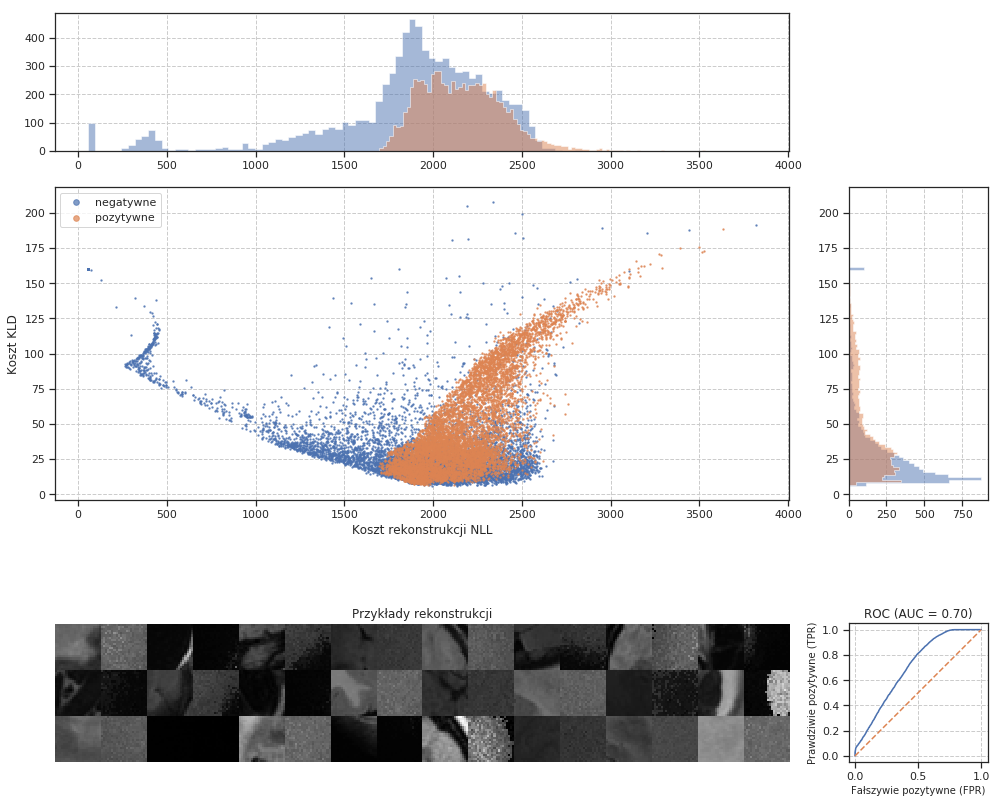
\includegraphics[width=1.0\textwidth]{images/soft_vae_v2}
    \caption{}
    \label{fig:soft_vae}
\end{figure}

\begin{figure}[h!]
    \centering
    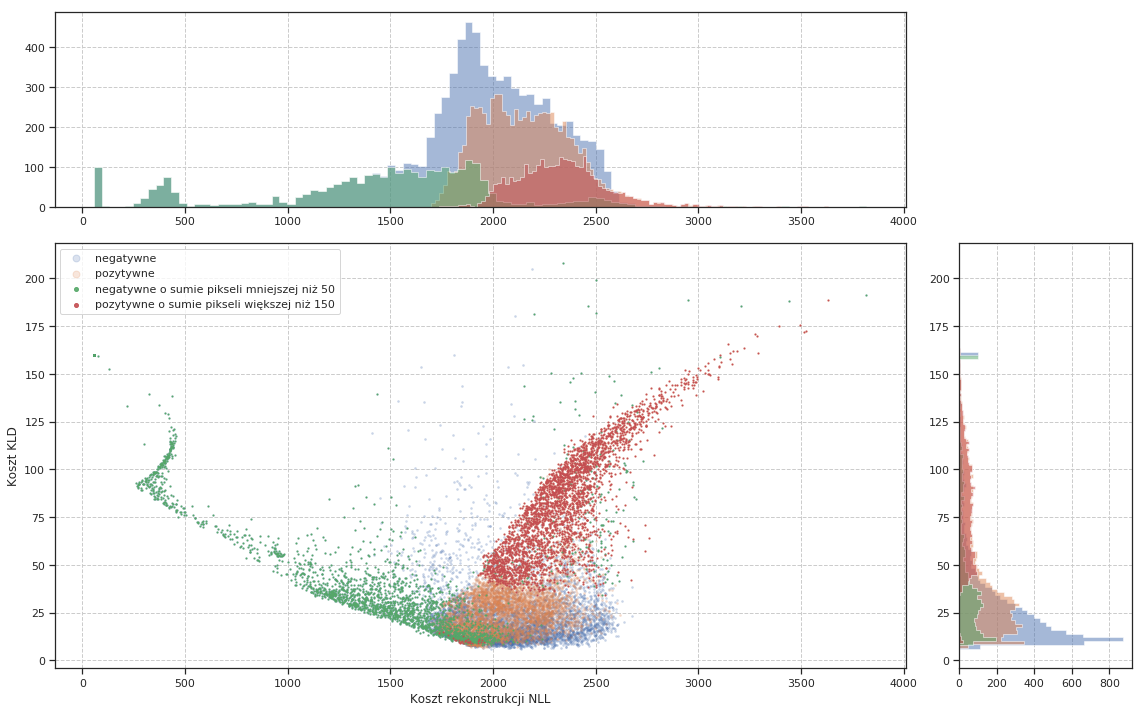
\includegraphics[width=1.0\textwidth]{images/soft_vae_th_v2}
    \caption{}
    \label{fig:soft_vae_th}
\end{figure}

\begin{figure}[h!]
    \centering
    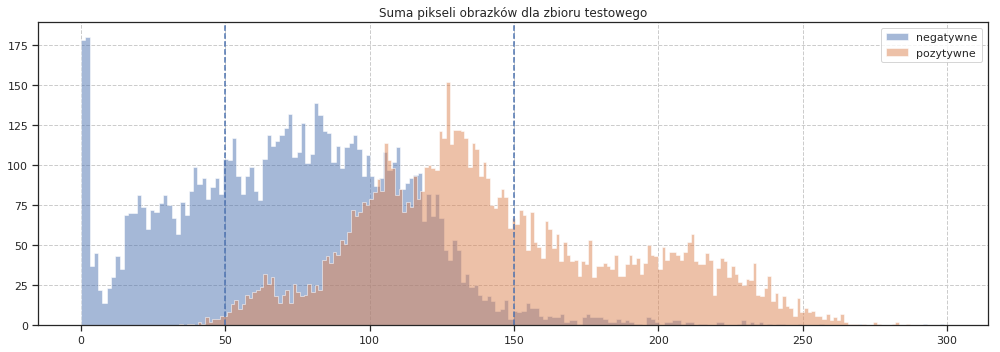
\includegraphics[width=1.0\textwidth]{images/pixels_hist_v2}
    \caption{}
    \label{fig:pixels_hist}
\end{figure}

\subsection{Wnioski}






\chapter{Podsumowanie}

\section{Wnioski}

Autoenkoder wariacyjny jest bardzo interesującym modelem bazującym na rachunku prawdopodobieństwa, który stara się je oddolnie oszacowywać dla wystąpienia danego zjawiska. Jest to przydatne w problemie znajdywania odchyleń w danych, co pokazałem na bazie prostego zbioru jakim jest MNIST. Niestety przy przejściu do bardziej skomplikowanych próbek, model ten nie był w stanie znaleźć na tyle znaczących cech, które byłyby wystarczające do wykrywania zaburzeń z zadowalającą precyzją. Może być kilka przyczyn wystąpienia tego zjawiska, zaczynając od zbyt słabego modelu jakim jest sam autoenkoder po niewystarczającą obróbkę danych.

\section{Usprawnienia}

Skoro wyszło, że model zwraca przede wszystkim uwagę na jasność obrazków, to można byłoby zastosować normalizację w postaci wyrównywania histogramu (ang. histogram equalization). Metoda ta pozwala na zwiększenie kontrastu próbki, a dodatkowo rozciąga występowanie piksli na całą przestrzeń przez co zmienia się ich łączna suma wartości. Można wyobrazić sobie, że jasne obrazki zrobią się ciemniejsze i odwrotnie w przeciwnym przypadku. Jest szansa, że zmusiło by to model to położenia nacisku na inne cechy.

Innym pomysłem mogłoby być usprawnienie obróbki danych poprzez ograniczenie się jedynie do najbardziej znaczącej zawartości czaszki jakim jest mózg. W danych na jednych obrazkach znajdują się dodatkowo oczy, a na innych nie. Są to jasne obiekty, co mogło wpłynąć na reprezentację danych. Dodatkowo sama czaszka w formie kości też jest rzadka, więc usunięcie takich nieistotnych danych pozwoliłoby na sensowne ograniczenie danych.

Problemem może być sam rozmiar wycinka i brak jakichkolwiek dodatkowych informacji. W tym momencie model tylko na bazie samego obrazka musi go dobrze zrekonstruować, co wydaje się bardzo trudne szczególnie w tych partiach przy krawędziach, o których ma najmniej danych. Rozwiązaniem mogłoby być dorzucenie dodatkowych informacji do dekodera o sąsiedztwie takiego wycinka, co mogłoby pozytywnie wpłynąć na koszt rekonstrukcji.



%\begin{thebibliography}{1}
%\bibitem{example} \ldots
%\end{thebibliography}

\end{document}
